\documentclass[twocolumn]{IEEEtran}
\usepackage{graphicx}
\usepackage[utf8x]{inputenc}
\usepackage{times}
\usepackage{amssymb,amsfonts}
\usepackage[tbtags]{amsmath}
\usepackage{cite}
\usepackage{slashbox}
\usepackage{pict2e}
\usepackage{float}
\usepackage[all]{xy}
\usepackage{graphics,graphicx,color,colortbl}
\usepackage{times}
\usepackage{subfigure}
\usepackage{wrapfig}
\usepackage{multicol}
\usepackage{cite}
\usepackage{url}
\usepackage[tbtags]{amsmath}
\usepackage{amsmath,amssymb,amsfonts,amsbsy}
\usepackage{bm}
\usepackage{algorithm}
\usepackage{algorithmic}
\usepackage[centerlast, small]{caption}
\usepackage[colorlinks=true, citecolor=blue, linkcolor=blue, urlcolor=blue,
breaklinks=true]{hyperref}

\begin{document}
\title{Uso de equipos del laboratorio e instrumentos de medida}
\author{José Fabio Lozano Ovalle Código: $222982$\\
	Wilson Orlando Macias Fuquen Código: $22$\\
	David Ricardo Martínez Hernández Código: $261931$}
\maketitle
\markboth{Universidad Nacional de Colombia}{}
\floatname{algorithm}{Algoritmo}
\begin{abstract}
En este informe se presentan los datos, observaciones y conclusiones obtenidos
durante la práctica de laboratorio, presentando los análisis correspondientes a
la información brindada por los fabricantes de los elementos de medición, de
igual medida se realiza el análisis del circuito resistivo.
\end{abstract}

\begin{keywords}
Alta Frecuencia, Baja Frecuencia, Corriente, Frecuencia, Multímetro, Onda Seno,
Onda Triangular, Osciloscopio, Potencia, Resistencias, Seguridad, Voltaje,
Voltaje de Offset, Voltaje Pico, Voltaje RMS.
\end{keywords}

\section{Objetivos}
\begin{itemize}
  \item Familiarizarse con los instrumentos de medición, conocer sus
características de funcionamiento y limitaciones.
  \item Conocer las normas básicas de seguridad en el laboratorio.
  \item Reforzar conceptos básicos de circuitos eléctricos, como valor pico,
RMS, forma de onda, entre otros. Utilizando al máximo los elementos de medida.
\end{itemize}

\section{Introducción}
\noindent
Un \textbf{circuito eléctrico} es una red cerrada de elementos en el que siempre
fluye constantemente una corriente eléctrica. La corriente es \textit{la razón
de cambio temporal de la carga que pasa por u punto dado}\footnote{Definición
tomada de \cite{dorf}, Página 8.}.
\begin{equation}
 i=\frac{dq}{dt}
  \label{equ1}
\end{equation}
\noindent
donde:\\
$q$ es la \textbf{carga} del electrón.\\
$t$ es el \textbf{tiempo}.\\
La unidad de corriente es el ampere (\textbf{A}).\\
Si la corriente a través de un elemento es constante se representa con la letra
\textbf{I}, una corriente constante se llama \textbf{corriente directa}.\\\\
El \textbf{voltaje} a través de un elemento es el trabajo necesario (energía
necesaria) para mover una carga eléctrica unitaria y positiva desde la terminal
$-$ hasta la terminal $+$\footnote{Definición tomada de \cite{dorf}, Página
15.}.
\begin{equation}
 v=\frac{dw}{dq}
  \label{equ2}
\end{equation}
donde:\\
$w$ es la \textbf{energía} o \textbf{trabajo} del electrón.\\
$q$ es la \textbf{carga} del electrón.\\
La unidad de voltaje es el volt (\textbf{V}).\\
Si el voltaje a través de un elemento es constante se representa con la letra
\textbf{V}, un voltaje constante se llama \textbf{voltaje directo}.\\\\
\textbf{Potencia} es la cantidad de energía entregada o absorbida en cierto
tiempo.\footnote{Texto tomado de \cite{dorf}, Página 15}
\begin{equation}
 p=\frac{dw}{dt}
\label{equ3}
\end{equation}
\noindent
donde:\\
$p$ es la potencia en watts.\\
$w$ es la energía en joules.\\
$t$ es el tiempo en segundos.
\begin{equation}
 p=\frac{dw}{dt}=\frac{dw}{dq}*\frac{dq}{dt}=i*v
\label{equ4}
\end{equation}
\noindent
\textbf{Valor de cresta o pico o máximo}: $V_m$ o $V_p$ Es la magnitud máxima
que toma la función en un instante de tiempo.\\
\textbf{Valor pico a pico o cresta a cresta}: $V_{pp}$ Es la magnitud de la
señal desde su amplitud mínima o negativa ($-Vm$) hasta su amplitud máxima o
positiva ($+Vm$). Para una señal simétrica el valor pico a pico es el doble del
valor máximo.\\
\textbf{Valor eficaz o valor rms (root mean square: raíz media cuadrática)}: Se
conoce que el voltaje en un toma corriente de una residencia debe ser de $120 \
V$ nominales, desde luego no es el valor medio, ni el valor pico, es el valor
eficaz o rms.\\
El valor rms es el valor equivalente al de una señal constante ($DC$) que
desarrollaría la misma potencia media ``P'' en un resistor ``R'' de
referencia.\\
Este valor rms es de sumo interés en los cálculos de potencia y
energía\footnote{Definiciones tomadas de \cite{page1}}.

\section{Materiales y Métodos}
\noindent
Para realizar esta práctica se necesito:
\begin{itemize}
  \item 9 resistencias de diferentes valores.
  \item Osciloscopio Hitachi.
  \item Dos Multímetros Fluke. Ref: 79 III True RMS Multimeter y 73 Series II
Multimeter.
  \item Un Multímetro UNIT UT33C.
  \item Genrador de funciones.
\end{itemize}

\section{Análisis y Resultados}
\noindent
\subsection{Medida de resistencias}
\noindent
Las resistencias utilizadas fueron $R_{1}=1 \ M \Omega$, $R_{2}=15 \ K \Omega$,
$R_{3}=120 \ K \Omega$, $R_{4}=200 \ \Omega$.
\begin{table}[H]
	\centering
\begin{tabular}[c]{|c|c|c|c|c|} \hline
\backslashbox{Escala}{Resistencia} & $R_{1}$ & $R_{2}$ & $R_{3}$ & $R_{4}$ \\
\hline
$2 \ M\Omega$ & 1.01 & 0.01 & 0.12 & 0.00 \\ \hline
$200 \ K\Omega$ & -- & 14.8 & 118.5 & 0.2 \\ \hline
$20 \ K\Omega$ & -- & 14.84 & -- & 0.20 \\ \hline
$2 \ K\Omega$ & -- & -- & -- & 198 \\ \hline
$200 \ \Omega$ & -- & -- & -- & 197.7 \\ \hline
\end{tabular}
	\caption{Valores de las resistencias medidas con el Multímetro
UNIT-UT33C}
	\label{tab1}
\end{table}
\noindent

Los valores medidos de las resistencias con el Fluke 73 fueron
\begin{table}[H]
	\centering
\begin{tabular}[c]{|c|c|c|c|c|} \hline
Resistencia & $R_{1}$ & $R_{2}$ & $R_{3}$ & $R_{4}$ \\ \hline
Valor & $1.009 \ M\Omega$ & $14.82 \ K\Omega$ & $118.4 \ K\Omega$ & $198.3 \
\Omega$ \\ \hline
\end{tabular}
	\caption{Valores de las resistencias medidas con el Multímetro Fluke 73
Series II}
	\label{tab2}
\end{table}
\noindent

Los valores medidos de las resistencias con el Fluke 79 fueron
\begin{table}[H]
	\centering
\begin{tabular}[c]{|c|c|c|c|c|} \hline
Resistencia & $R_{1}$ & $R_{2}$ & $R_{3}$ & $R_{4}$ \\ \hline
Valor & $1.008 \ M \Omega$ & $14.84 \ K\Omega$ & $118.4 \ K\Omega$ & $198.8 \
\Omega$ \\ \hline
\end{tabular}
	\caption{Valores de las resistencias medidas con el Multímetro Fluke 79
III True RMS Multimeter}
	\label{tab3}
\end{table}
\noindent
De acuerdo con la tolerancia proporcionada por el fabricante las resistencias se
encuentran dentro de este rango.\\
Los elementos con los cuales se midieron las resistencias pueden afectar la
exactitud de las mismas.

\subsection{Circuito Serie-Paralelo}
\noindent
El circuito que se realizo fue el mostrado en la figura \ref{fig1}, con $V_{F}=5
\ V$, $R_{1}=2.2 \ K \Omega$, $R_{2}=1 \ K \Omega$, $R_{3}=10 \ K \Omega$,
$R_{4}=1 \ K \Omega$ y $R_{5}=20 \ K \Omega$.
\begin{figure}[H]
	\centering
		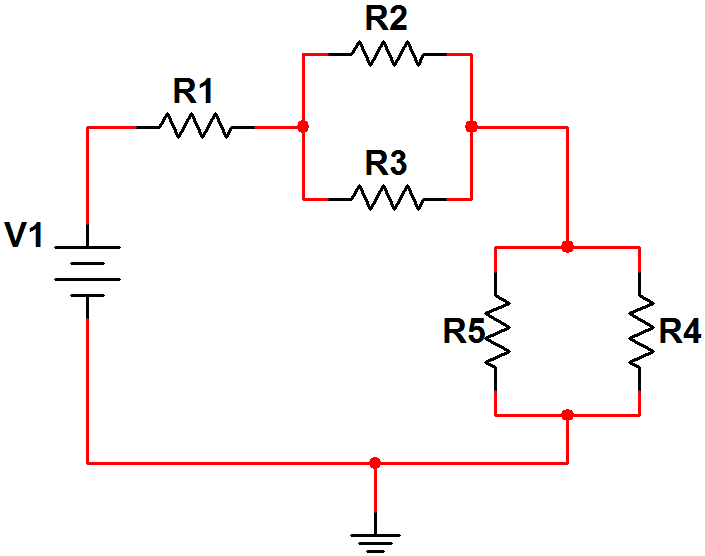
\includegraphics[scale=0.35]{circuit.png}
	\caption{Circuito Serie-Paralelo}
	\label{fig1}
\end{figure}
\noindent
\begin{table}[H]
	\centering
\begin{tabular}[c]{|c|c|c|c|} \hline
 & Voltaje ($V$) & Corriente ($mA$) & Osciloscopio \\ \hline
$V_{Fuente}$ & 5.01 & 1.245 & 5.2 2$V/Div$ \\ \hline
$V_{R_{1}}$ & 2.713 & 1.245 & 2.8 1$V/Div$ \\ \hline
$V_{R_{2}}$ & 1.117 & 1.132 & 1.1 0.5$V/Div$ \\ \hline
$V_{R_{3}}$ & 1.117 & 0.113 & 1.1 0.5$V/Div$ \\ \hline
$V_{R_{4}}$ & 1.178 & 1.183 & 1.2 0.5$V/Div$ \\ \hline
$V_{R_{5}}$ & 1.178 & 0.060 & 1.2 0.5$V/Div$ \\ \hline
\end{tabular}
	\caption{Valores obtenidos por el circuito por medio del Multímetro 79 y
el osciloscopio Hitachi}
	\label{tab4}
\end{table}
\noindent

\subsection{Generador de Funciones Onda Seno}
\noindent
Se realizo el circuito de la fig \ref{fig2}, con dos valores de frecuencia
diferentes y un componente DC. Para alta frecuencia se utilizó una frecuencia de
$5 \ KHz$, para el de baja frecuencia se utilizó una frecuencia de $500 \ Hz$ y
finalmente para el componente DC se utilizó una frecuencia de $5 \ KHz$.
\begin{figure}[H]
	\centering
		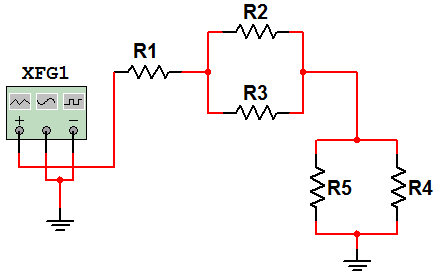
\includegraphics[scale=0.5]{circuit_2.png}
	\caption{Circuito Serie-Paralelo}
	\label{fig2}
\end{figure}

\subsubsection{Alta frecuencia}
Los valores obtenidos
\begin{table}[H]
	\centering
\begin{tabular}[c]{|c|c|c|c|} \hline
 & Voltaje ($V$) & Corriente ($mA$) & Osciloscopio \\ \hline
$V_{Fuente}$ & 5.01 & 1.238 & 7.8 2$V/Div$ \\ \hline
$V_{R_{1}}$ & 2.693 & 1.238 & 6.8 2$V/Div$ \\ \hline
$V_{R_{2}}$ & 1.112 & 1.125 & 2.0 2$V/Div$ \\ \hline
$V_{R_{3}}$ & 1.112 & 0.113 & 2.0 0.5$V/Div$ \\ \hline
$V_{R_{4}}$ & 1.172 & 1.178 & 1.7 0.5$V/Div$ \\ \hline
$V_{R_{5}}$ & 1.172 & 0.061 & 1.7 0.5$V/Div$ \\ \hline
\end{tabular}
	\caption{Valores obtenidos por el circuito por medio del Multímetro 79 y
el osciloscopio Hitachi}
	\label{tab5}
\end{table}

\subsubsection{Baja frecuencia}
Los valores obtenidos
\begin{table}[H]
	\centering
\begin{tabular}[c]{|c|c|c|c|} \hline
 & Voltaje ($V$) & Corriente ($mA$) & Osciloscopio \\ \hline
$V_{Fuente}$ & 4.98 & 1.234 & 7.2 2$V/Div$ \\ \hline
$V_{R_{1}}$ & 2.682 & 1.234 & 6.6 2$V/Div$ \\ \hline
$V_{R_{2}}$ & 1.108 & 1.121 & 2.0 2$V/Div$ \\ \hline
$V_{R_{3}}$ & 1.108 & 0.113 & 2.0 0.5$V/Div$ \\ \hline
$V_{R_{4}}$ & 1.167 & 1.174 & 1.7 0.5$V/Div$ \\ \hline
$V_{R_{5}}$ & 1.167 & 0.060 & 1.7 0.5$V/Div$ \\ \hline
\end{tabular}
	\caption{Valores obtenidos por el circuito por medio del Multímetro 79 y
el osciloscopio Hitachi}
	\label{tab6}
\end{table}
\noindent

\subsubsection{Componente DC}
Onda senoidal de 5 KHz con un $V_{offset}=2.006 \ V$
\begin{table}[h]
	\centering
\begin{tabular}[c]{|c|c|c|c|c|} \hline
 & $V_{DC}$ & $V_{AC}$ & $I_{DC}$ & $I_{AC}$ \\ \hline
$V_{Fuente}$ & 1.748 & 4.99 & 0.435 & 1.237 \\ \hline
$V_{R_{1}}$ & 0.948 & 2.683 & 0.435 & 1.237 \\ \hline
$V_{R_{2}}$ & 0.390 & 1.108 & 0.393 & 1.120 \\ \hline
$V_{R_{3}}$ & 0.390 & 1.108 & 0.040 & 0.133 \\ \hline
$V_{R_{4}}$ & 0.411 & 1.167 & 0.414 & 1.177 \\ \hline
$V_{R_{5}}$ & 0.411 & 1.167 & 0.020 & 0.060 \\ \hline
\end{tabular}
	\caption{Valores obtenidos por el circuito por medio del Multímetro 79 y
el osciloscopio Hitachi}
	\label{tab7}
\end{table}
\noindent

\subsection{Generador de Funciones Onda Triangular}
\noindent
\begin{table}[H]
	\centering
\begin{tabular}[c]{|c|c|c|c|} \hline
 & Voltaje ($V$) & Corriente ($mA$) & Osciloscopio \\ \hline
$V_{Fuente}$ & 4.29 & 1.063 & 7.8 2$V/Div$ \\ \hline
$V_{R_{1}}$ & 2.305 & 1.063 & 6.8 1$V/Div$ \\ \hline
$V_{R_{2}}$ & 0.951 & 0.966 & 2.2 1$V/Div$ \\ \hline
$V_{R_{3}}$ & 0.951 & 0.097 & 2.2 1$V/Div$ \\ \hline
$V_{R_{4}}$ & 1.003 & 1.011 & 1.8 0.5$V/Div$ \\ \hline
$V_{R_{5}}$ & 1.003 & 0.052 & 1.8 0.5$V/Div$ \\ \hline
\end{tabular}
	\caption{Valores obtenidos por el circuito por medio del Multímetro 79 y
el osciloscopio Hitachi}
	\label{tab8}
\end{table}

\section{Peguntas}
\begin{enumerate}
  \item ¿Que tanto varia el valor de resistencia medido experimentalmente con
respecto al mencionado por el fabricante?. ¿Se encuentra dentro de la
tolerancia?\\
Los valores medidos experimentalmente de cada resistencia se encuentran
consignados en la TABLA \ref{tab1}, se puede observar que se encuentran entre el
rango de tolerancia suministrado por el fabricante, siendo de un $\pm 5\%$.
  \item ¿Que diferencia existe entre los valores de tensión y corriente medidos
con un osciloscopio, un multímetro y la teoría?\\
Los valores medidos con osciloscopio son valores pico para tensión, además no se
puede medir corriente con el osciloscopio de manera directa para ello se utiliza
la ley de Ohm.\\
Los valores obtenidos con un multímetro son valores \textbf{RMS} (\textit{Root
Mean Square}) ó valores efectivos tanto para corriente como para voltaje; estos
valores son manejados al realizar cálculos teóricos en \textbf{AC}. Los cálculos
teóricos no tiene en cuenta las incertidumbres asociadas a los elementos
utilizados para la práctica.
  \item ¿Que limitaciones tienen los equipos en cuanto a formas de onda y
frecuencia en la práctica?. ¿Concuerda con el fabricante?\\
\textbf{Osciloscopio}: Para evaluar la calidad del osciloscopio a utilizar se
deben seguir los siguientes parámetros:
\begin{itemize}
 \item Ancho de Banda: Especifica el rango de frecuencias que el osciloscopio
puede medir con precisión. Por convención el ancho de banda se calcula desde $0
\ Hz$ hasta $20 \ MHz$ dependiendo de su resolución.
 \item Tiempo de Subida: Este parámetro sirve para determinar el tiempo de
respuesta del osciloscopio con respecto a la señal medida. Un osciloscopio no
puede visualizar pulsos con tiempos de subida más rápidos que el suyo propio.
 \item Sensibilidad Vertical: Es una característica que posee el instrumento
para detectar rangos de voltajes muy bajos o altos. Se suele proporcionar en $V$
o $mV$ por división vertical desde $2 \ mV/div$ hasta $5 \ V/div$ en este caso.
 \item Resolución Vertical: Se mide en bits y es un parámetro que da la
resolución del conversor $A/D$ del osciloscopio digital. Que indica con que
precisión se convierten las señales de entrada en valores digitales almacenados
en la memoria. Técnicas de cálculo pueden aumentar la resolución efectiva del
osciloscopio.
 \item Velocidad de Muestreo: Para osciloscopios análogos esta característica
indica la velocidad máxima del barrido horizontal, lo que permitirá observar
sucesos más rápidos. Suele ser del orden de nanosegundos por división
horizontal.
 \item Exactitud de la Base de Tiempos: Indica la precisión en la base de
tiempos del sistema horizontal del osciloscopio para visualizar el tiempo.
\end{itemize}
\noindent
\textbf{Multímetro Digital}: Este dispositivo hace medidas de corriente o
voltaje por medio de la conversión de la señal a su correspondiente valor
\textbf{RMS}. Los multímetros de respuesta promedio son calibrados para lecturas
correctas solo en ondas sinusoidales, y darán lectura incorrecta en otro tipo de
señales.\\
Algunos dispositivos más costosos incluirán el valor RMS de diferentes tipos de
formas de onda; el manual de usuario para el multímetro indicara los límites del
factor de cresta y frecuencia para la cual la calibración de este es válida. Las
limitaciones de frecuencia superior de multímetros digitales varían de $20 \
KHz$ a más de $300 \ KHZ$ dependiendo del modelo. Sus limitaciones de frecuencia
pueden ser corregidas considerablemente mediante el uso de circuitos asociados.
  \item ¿Que valor arroja el multímetro cuando mide una señal AC$+$DC?\\
Si el multímetro se encuentra midiendo DC mostrara el valor de Offset de la
señal. Si el multímetro se encuentra midiendo AC mostrara el valor RMS de señal.
  \item ¿Que valor arroja el multímetro cuando mide una señal triangular?\\
Si el multímetro es de baja gama arrojara el valor promedio para una onda
sinusoidal. De lo contrario indicara valores erróneos.
\begin{equation}
V_{RMS}=\frac{V_{pico}}{\sqrt{2}} 
\end{equation}
\noindent
Si mide valores efectivos verdaderos arrojará un dato muy preciso que
corresponde al valor RMS.
\begin{equation}
{F_{rms}} = \sqrt {\frac{1}{T}\int\limits_0^T {{f^2}\left( t \right)} dt}
\end{equation}
  \item Teniendo en cuenta las tolerancias de los elementos ¿Cuál puede ser el
error esperado en las mediciones?\\
Los errores estimados para esta práctica son:
\begin{itemize}
 \item Tolerancia de las resistencias
 \item Tolerancia de la fuente
 \item Tolerancia del multímetro
 \item Temperatura
 \item Estabilidad de la red
 \item Protoboard, cables, sondas, entre otros
\end{itemize}
\noindent
De los cuales se pueden omitir los siguientes:
\begin{itemize}
 \item Temperatura
 \item Estabilidad de la red
 \item Protoboard, cables, sondas, entre otros
\end{itemize}
\noindent
dado que pertenecen a los errores del tipo B.\\
\noindent
Para obtener el error es necesario hallar el intervalo de confianza  de cada
elemento. En seguida se hace la propagación de la incertidumbre, finalmente se
utiliza la ecuación de error medio.
\begin{equation}
 {\exists _\% } = \frac{{\left| {Valo{r_{Terico}} - Valo{r_{Practico}}}
\right|}}{{Valo{r_{Teorico}}}}*100\% 
\end{equation}
  \item ¿Que diferencia existe al medir con uno canal y con los dos canales del
osciloscopio al mismo tiempo?\\
Con un canal se puede visualizar solo una señal al tiempo; el disponer de dos
canales permite comparar señales de forma muy cómoda, y buscar relaciones de
fase y amplitudes que puedan haber entre estas, por ejemplo, aplicando cada una
de las señales, a las entradas ``X'' e ``Y'' del osciloscopio y en el caso de
que exista una relación armónica completa entre ambas, se introduce en la
pantalla una de las llamadas ``figuras de Lissajous'', a la vista de la cual se
pueden averiguar el numero de veces que una frecuencia contiene a la otra y por
lo tanto deducir el valor de la frecuencia desconocida.\\
En cuanto a la conexión, cuando se vayan a medir $2$ señales diferentes
procedentes de un mismo circuito, se debe tener un cuidado especial con la
conexión a tierra, ya que si el osciloscopio, y las señales de entrada se
encuentran referenciadas con la misma tierra, es posible que exista un error en
la representación de una de las $2$ señales de entrada.
\end{enumerate}

\section{Seguridad Industrial}
\noindent
No se debe trabajar solo porque si ocurre un accidente no tiene apoyo ni
asistencia, no debe llevar objetos metálicos en las manos o brazos y si posee
algun tipo de material conductor en su cuerpo notificarlo a su equipo de
trabajo.\\
Establecer puestas a tierra para descargar la energía eléctrica estática
presente en el cuerpo de los integrantes del grupo y así evitar daños a la
integridad física, del circuito y de los mismos.\\
Utilizar prendas adecuadas para realizar el trabajo en el laboratorio.\\
Identificar la ruta de evacuación y elementos de seguridad previamente a la
práctica para poder utilizarla en caso de emergencia.\\
Identificar y utilizar los elementos de protección personal para evitar
accidentes.\\
Des energizar los elementos a utilizar y asegurarse que el último elemento a
utilizar sea la fuente.\\
En los posible estar inscrito a EPS, ARP, Poliza de seguros, etc, según sea el
caso.

\section{Conclusiones}
\begin{itemize}
  \item El error solo se puede calcular al haber realizado la práctica dado que
se debe comparar con el valor teórico, realizando la propagación de la
incertidumbre y calculando el error esprado.
  \item Dependiendo del análisis deseado se puede trabajar con multímetros, los
cuales miden valores RMS u osciloscopio para realizar un análisis de forma de
onda y frecuencia.
  \item Dependiendo del tipo de miltímetro y la forma de onda de la señal,
genera diferentes tipos de problemas al realizar las mediciones deseadas.
  \item Es necesario conocer las características de cada elemento, para
seleccionar adecuadamente los equipos y realizar una correcta medición.
\end{itemize}

\bibliographystyle{ieeetran}
\begin{thebibliography}{99}
\bibitem{dorf} Dorf  \& Svoboda.
{\em "`Circuitos Eléctricos"'}.
Alfaomega, Sexta Edición, 2006.

\bibitem{page1}
\url{http://publico.ing.ues.edu.sv/asignaturas/ael115/Unidad-III%20AC/3-1%20Valor%20m
edio%20y%20eficaz%20(rms).pdf}
\end{thebibliography}
\end{document}